% !TEX root = ../my-thesis.tex
%
\chapter{Data Analysis}
\label{sec:analysis}
In this chapter the models calculated for each country are reviewed. First, a look at the standardised incidence rate for each country is taken, before spatial models, spatio-temporal models and finally regression models are discussed.
\section{Standardised Incidence Ratio}
This section takes a brief look at the standardised incidence ratio for the countries of interest.
\subsection{Standardised Incidence Ratio for Germany}
When looking at the standardised incidence ratio for Germany, it is noticeable that the actual number of infections in the eastern parts of Germany, especially in Saxony, is considerably higher than the expected number of infections. Furthermore, parts of Bavaria have an increased standardised incidence ratio compared to the rest of Germany, excluding Saxony, see Figure~\ref{sirgermany}
% \begin{figure}[H]
%   \centering
%   \includesvg[width = 1.2\textwidth]{sir_germany.svg}
%   \caption{The standardised incidence ratio for Germany based on the data of the 5th of March 2021}
%   \label{sirgermany}
% \end{figure}
\begin{figure}[H]
  \centering
  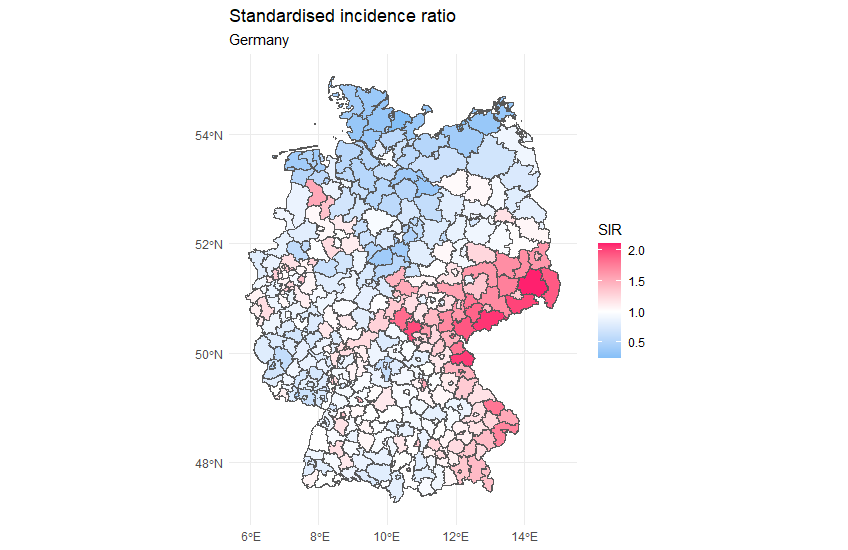
\includegraphics[width = 1.2\textwidth]{sir_germany.png}
  \caption{The standardised incidence ratio for Germany based on the data of the 5th of March 2021}
  \label{sirgermany}
\end{figure}
\subsection{Standardised Incidence Ratio for Norway}
Looking at the standardised incidence rate for Norway, a standardised incidence rate of less than 1 can be seen for most municipalities north of Trondheim. In the southern parts of Norway there are several municipalities with a rate above 1, for example the standardised incidence rate around the capital Oslo is around 2. However, the two small municipalities, Hyllestad and Ulvik, have the highest standardised incidence rate in Norway. The SIR in Hyllestad is around 5, following an outbreak in a shipyard in autumn 2020 \cite{newspaper1}, while Ulvik has a ratio of around 9, following an outbreak of the UK variant of Covid-19. According to the head of the municipality, Hans Petter Thorbjørnsen, the infections are thought to have spread through children \cite{newspaper2}. See Figure~\ref{sirnorway} for more information.
% \begin{figure}[H]
%   \centering
%   \includesvg[width = 1.2\textwidth]{sir_norge.svg}
%   \caption{The standardised incidence ratio for Norway based on the data of the 5th of March 2021}
%   \label{sirnorway}
% \end{figure}
\begin{figure}[H]
  \centering
  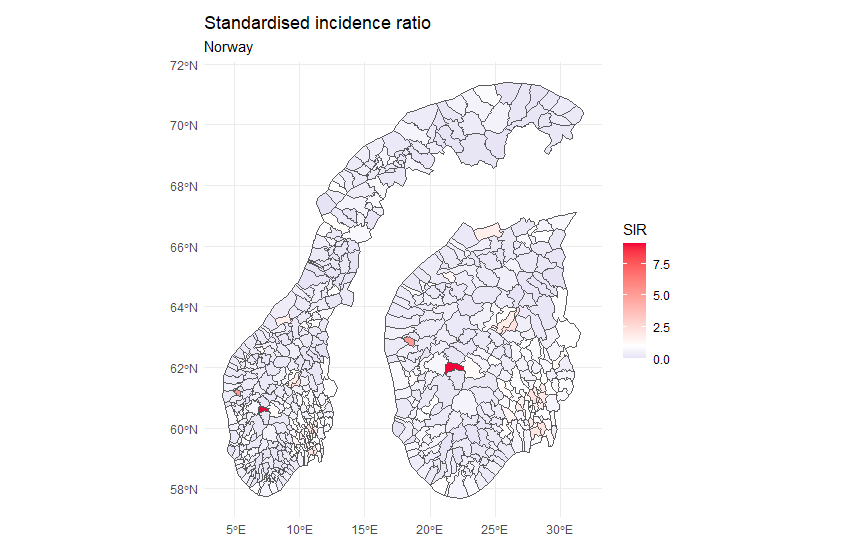
\includegraphics[width = 1.2\textwidth]{sir_norge.png}
  \caption{The standardised incidence ratio for Norway based on the data of the 5th of March 2021}
  \label{sirnorway}
\end{figure}
\clearpage
\section{Spatial Models}
After looking at the standardised incidence rates for the countries of interest, the next step is to take a closer look at the current figures for the respective countries. Spatial models are used to try to extract the factors that cause some populations to be at higher risk than other populations. Four different types of models are used for each country:
\begin{itemize}
    \item[1.] The Besarg-Yollie-Mollie Model
    \item[2.] Besags Proper Spatial Model
    \item[3.] The Leroux-Model
\end{itemize}
Three measures are used to compare the models, the DIC, the WAIC and the CPO. \\
Before the models are computed, however, the distribution that fits the number of cases must first be found. For this, the function \texttt{descdist()} from the \texttt{fitdistrplus} R package is used. With this function, descriptive parameters of an empirical distribution can be calculated and a skewness-kurtosis plot is provided. The plots for Germany and Norway can be seen in Figure~\ref{cf_germany} and Figure~\ref{cf_norge}.
% \begin{figure}[H]
%     \centering
%     \includesvg[width = 0.8\textwidth]{cf-germany.svg}
%     \caption{The Cullen and Frey graph for Germany}
%     \label{cf_germany}
% \end{figure}
\begin{figure}[H]
    \centering
    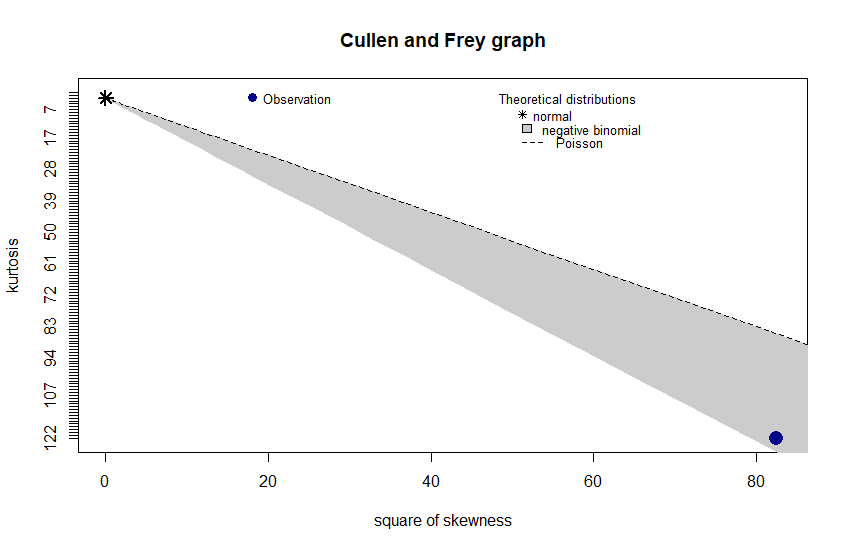
\includegraphics[width = 0.8\textwidth]{cf-germany.png}
    \caption{The Cullen and Frey graph for Germany}
    \label{cf_germany}
\end{figure}
% \begin{figure}[H]
%     \centering
%     \includesvg[width = 0.8\textwidth]{cf_norge.svg}
%     \caption{The Cullen and Frey graph for Norway}
%     \label{cf_norge}
% \end{figure}
\begin{figure}[H]
    \centering
    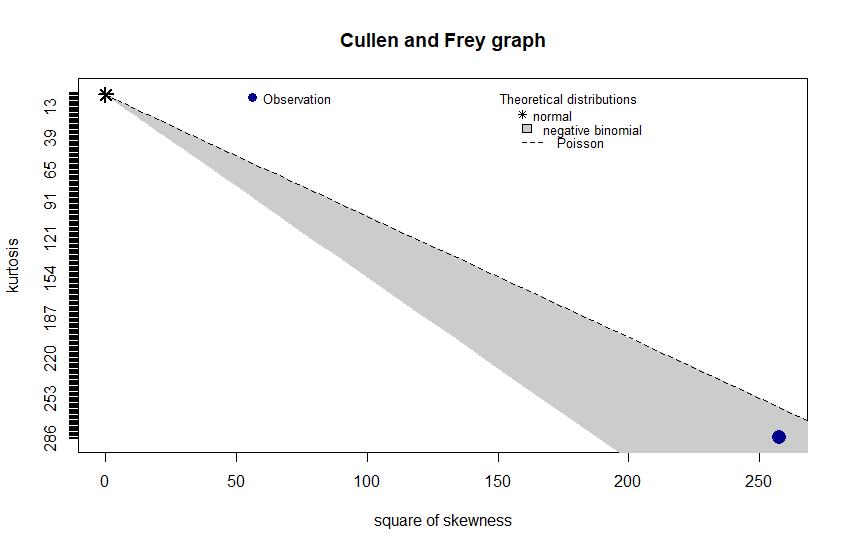
\includegraphics[width = 0.8\textwidth]{cf_norge.png}
    \caption{The Cullen and Frey graph for Norway}
    \label{cf_norge}
\end{figure}
Following these plots, a negative binomial distribution is fitted to the data using the maximum likelihood method. The function \texttt{fitdist()} is used for this. The fits can be seen in Figure~\ref{nb_germany} and Figure~\ref{nb_norge}.
% \begin{figure}[H]
%     \centering
%     \includesvg[width = 0.8\textwidth]{neg_binom_germany.svg}
%     \caption{A negative binomial fit to the number of cases in German municipalities}
%     \label{nb_germany}
% \end{figure}
\begin{figure}[H]
    \centering
    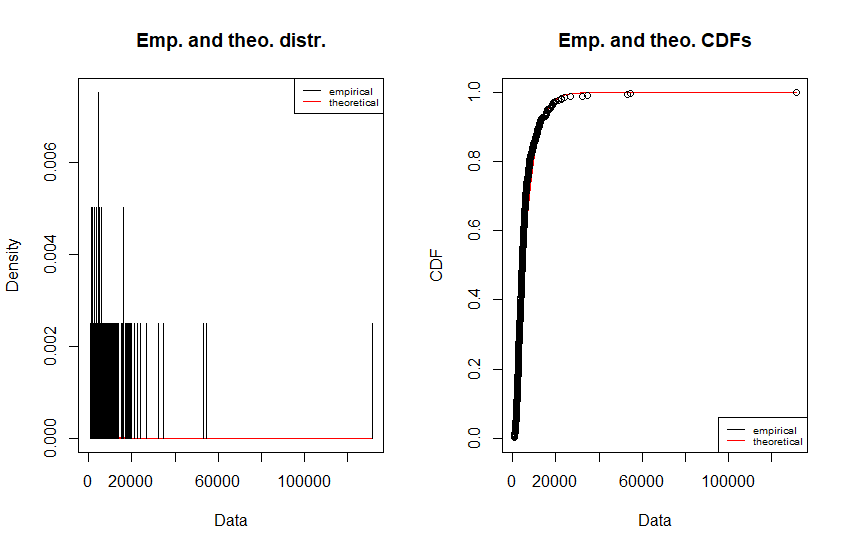
\includegraphics[width = 0.8\textwidth]{neg_binom_germany.png}
    \caption{A negative binomial fit to the number of cases in German municipalities}
    \label{nb_germany}
\end{figure}
% \begin{figure}[H]
%     \centering
%     \includesvg[width = 0.8\textwidth]{neg_binom_norge.svg}
%     \caption{A negative binomial fit to the number of cases in Norwegian municipalities}
%     \label{nb_norge}
% \end{figure}
\begin{figure}[H]
    \centering
    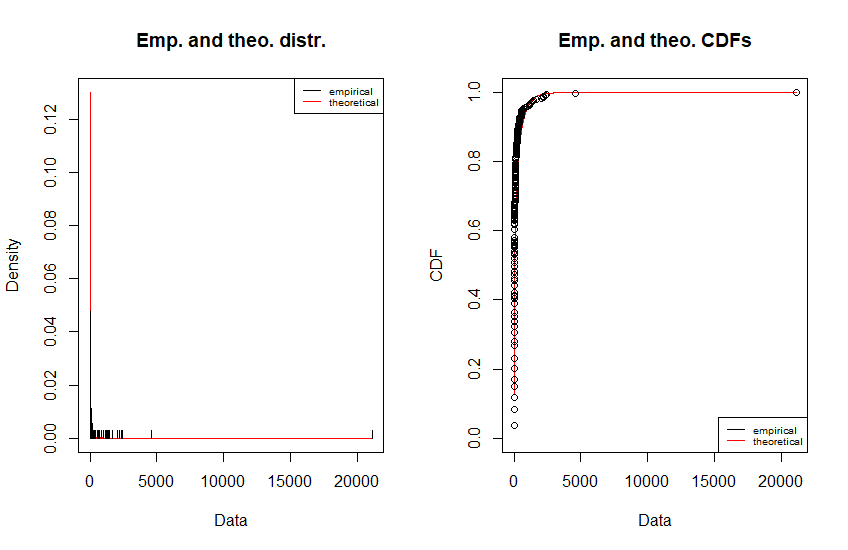
\includegraphics[width = 0.8\textwidth]{neg_binom_norge.png}
    \caption{A negative binomial fit to the number of cases in Norwegian municipalities}
    \label{nb_norge}
\end{figure}
Lastly, the AIC was calculated for fitting a normal distribution to the data, a Poisson distribution to the data and a negative binomial distribution to the data. The values can be seen in Table~\ref{aic}. Afterwards, the negative binomial distribution was chosen as the distribution of the target variable in both cases. \\
\begin{table}[H] 
\caption{THE AIC for different distributions for Germany and Norway \label{aic}}
\begin{tabular}{l l r}
\toprule
\textbf{Country}	& \textbf{Distribution}	& \textbf{AIC} \\
\midrule
Germany & Normal & 8364 \\
Germany & Poisson & 2065103 \\
Germany & Negative Binomial & 7726 \\
Norway & Normal & 6052 \\
Norway & Poisson & 314100 \\
Norway & Negative Binomial & 4018 \\
\bottomrule
\end{tabular}
\end{table}
For all countries, the models were computed with
\begin{itemize}
    \item[1.] only the demographic variables as covariates
    \item[2.] only the infrastructural variables as covariates
    \item[3.] both, demographic and infrastructural variables, as covariates
    \begin{itemize}
        \item[3.1] Without variable selection
        \item[3.2] With variable selection
    \end{itemize}
\end{itemize}
For each model type, different values for the penalised prior component were tried. As this resulted in a large number of models, only the model with the best performance for each model class is examined in more detail. To decide which models perform best, the DIC, WAIC and CPO are used. A list of all calculated models along with their performance measures is provided in the appendix.
\subsection{Spatial Models for Germany}
First, a look is taken at the spatial models calculated for Germany. All models are run with the INLA \cite{rinla} R package.\\
To specify a BYM2-2 model in R, the following code can be used:
\begin{lstlisting}[language=R]
# Specify a prior distribution
prior_1 <- list(
  prec = list(
    prior = "pc.prec",
    param = c(1, 0.01)
  )
)
# Create a neighbourhood list
nb <- poly2nb(newest_numbers_germany)
# save the neighbourhood
nb2INLA("maps/map_2.adj", nb)
# load it
g <- inla.read.graph(filename = "maps/map_2.adj")
# specify the model formula
formula_1 <- CumNumberTestedIll ~
  # add the demographic vars and pop density
  pop_dens + urb_dens + sex + 
  # specify the model with neighbourhood matrix
  f(
    idarea_1, model = "bym2", graph = g,
    scale.model = TRUE, hyper = prior_1
  ) +
  # add a random effect to the model
  f(idarea_2, model = "iid")
# compute the model
res_1 <- inla(
  formula_1,
  family = "nbinomial",
  data = newest_numbers,
  E = expected_count,
  control.predictor = list(
    compute = TRUE
  ),
  control.compute = list(dic = TRUE, waic = TRUE, cpo = TRUE)
)
\end{lstlisting}
In the example above, a random effect is added to the model. As this random effect can sometimes cover the true effects however, all models were computed without such an effect.
% SCHREIB WIE DU DAS MIT DEN RANKS GEMACHT HAST DU IDIOT
\subsubsection{Demographic Models}
The best performing model based on demographic variables was a Leroux model that was computing using the following formula:
\begin{lstlisting}[language=R]
formula_7_leroux <- CumNumberTestedIll ~
  pop_dens + urb_dens + sex + trade_tax + income_total +
  f(
    idarea_1, model = "generic1", Cmatrix = C,
    hyper = prior_1
  )
\end{lstlisting}
The performance measure of this model and the best performing BYM2 and Besag proper model are shown in Table~\ref{demoGermany}. In total, 45 models were computed. The Leroux model was the best in terms of DIC and it also performed well in terms of the CPO. In fact, the 15 best models in terms of the CPO were all Leroux models. The best BYM2 model showed good performance in terms of the DIC and WAIC whereas Besags proper spatial model only showed good performance in terms of the WAIC.
\begin{table}[H] 
\caption{The performance measures for the best performing demographic model of each type. The rank in terms of each performance measure is denoted in the brackets. \label{demoGermany}}
\begin{tabular}{l l l l}
\toprule
\textbf{Model}	& \textbf{DIC}	& \textbf{WAIC} & \textbf{CPO} \\
\midrule
Leroux & 5598 (1) & 5665 (20) & -3818 (7) \\
BYM2 & 5630 (5) & 5576 (3) & -3343 (30)\\
Besags Proper  & 5680 (17) & 5604 (7) & -3334 (34) \\
\bottomrule
\end{tabular}
\end{table}
The fixed effects summaries are presented in Table~\ref{fixedDemoGermany}. By exponentiating the coefficients, they can more easily be interpreted. To get these values, the following code can be used:
\begin{lstlisting}[language=R]
# get the exponentiated value
inla.emarginal(exp, model_7_leroux$marginals.fixed$pop_dens)
# calculate the increase in risk if the 
# population ensity increases by 100
inla.emarginal(
  exp,
  model_7_leroux$marginals.fixed$pop_dens
  ) ^ 100
\end{lstlisting}
\begin{table}[H] 
\caption{The fixed effects for model 9. Values are rounded. \label{fixedDemoGermany}}
\begin{tabular}{l r r r r}
\toprule
\textbf{Variable}	& \textbf{Mean}	& \textbf{exp(mean)} \\
\midrule
(Intercept) & 2.77 & 42.6\\
pop\_dens & 0.00012 & 1.000125\\
urb\_dens &  -0.00091 & 0.999\\
sex & -5.25 & 0.252\\
trade\_tax & 0.00000053& 1.000001 \\
income\_total & -0.000015 & 0.999\\
\bottomrule
\end{tabular}
\end{table}
From this summary it can be seen that if the population density or the income by trade tax increases the relative risk of getting increases as well. An increase of 100 in terms of the population density leads to around a 1.01\% higher risk of getting infected and an increase of 20000€ / 1000 inhabitants leads to a 1.01\% increase in the risk of getting infected. \\
However having a higher income overall decreases the risk of infection, therefore people living in economically poorer regions of Germany have a greater risk of contracting the virus. An increase in total income by 1000€ / 1000 inhabitants decreases the infection risk by around 1.6\%. A higher urban density too slightly decreases the risk of contracting Covid-19, for instance an increase by 10 in urban density leads to a decrease in the relative risk by 1\%. Lastly, regions with a higher proportion of females living there are at a lower risk of infection, as an increase in the female proportion by 0.01 leads to a risk decrease of 1.4\%. \\
A plot of the relative risk is shown in Figur~\ref{relriskDemoGermany}
% \begin{figure}[H]
%     \centering
%     \includesvg[width = 0.8\textwidth]{demo_germany.svg}
%     \caption{The relative risk for contracting Covid-19 based on demographic variables}
%     \label{relriskDemoGermany}
% \end{figure}
\begin{figure}[H]
    \centering
    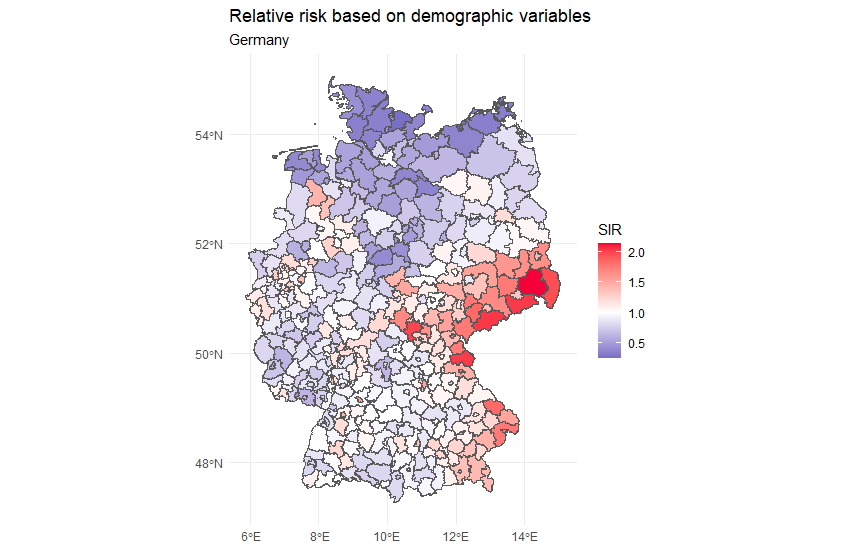
\includegraphics[width = 0.8\textwidth]{tex_files/demo_germany.png}
    \caption{The relative risk for contracting Covid-19 based on demographic variables}
    \label{relriskDemoGermany}
\end{figure}
\textbf{Models Based on the Infrastructure Variables} \\
The best performing model based on the infrastructural variables used the following formula and achieved the following performance:
\begin{lstlisting}[language=R]
formula_11 <- CumNumberTestedIll ~
  marketplace + entertainment + sport + clinic + toilet +
  hairdresser + shops + place_of_worship + retail + nursing_home +
  restaurant + aerodrome + office + university + platform +
  schools + college + banks + kindergarten + bakeries +
  gas + atm +
  f(
    idarea_1, model = "bym2", graph = g,
    scale.model = TRUE, hyper = prior_1
  )
\end{lstlisting}
\begin{table}[H] 
\caption{The performance measures for model 1 and 11\label{model11}}
\begin{tabular}{l r r r}
\toprule
\textbf{Model}	& \textbf{DIC}	& \textbf{WAIC} & \textbf{CPO} \\
\midrule
Model 1 & 5637 & 5581 & -3358 \\
Model 11 & 5687 & 5653 & -3367 \\
\bottomrule
\end{tabular}
\end{table}
This model performed worse in terms of both the DIC and WAIC, but better than the first model in terms of the CPO. \\
The fixed effects summaries are shown in Table~\ref{fixed11}. The intercept for this model is lower due to the addition of more variables to the model. The four main driving factors for higher risk of contracting Covid-19 are marketplaces; entertainment venues, defined as cinemas, theatres and nightclubs; airports; and shops. Since both marketplaces and entertainment venues tend to attract large audiences, it is perhaps not surprising that a greater number of these establishments leads to a higher risk of contracting a viral disease. The same is true for shops which are defined as supermarkets, convenience stores and drugstores, also resulting in a higher risk of becoming infected, although it is lower than for marketplaces and places of entertainment. Aerodromes too result in a higher risk of infection, as many people congregate here as well, and potentially people coming from risk areas. Gas stations and banks, on the other hand, reduce the risk the most. However, this does not necessarily mean that these types of buildings make an area safer.
\begin{table}[H] 
\caption{The fixed effects for model 11. Values are rounded. Not all variables are included\label{fixed11}}
\begin{tabular}{l r r r r}
\toprule
\textbf{Variable}	& \textbf{Mean}	& \textbf{SD} \\
\midrule
(Intercept) & 0.081 & 0.10 \\
marketplace & 1.11 & 0.71 \\
aerodrome & 0.43 & 0.68 \\
entertainment & 0.42 & 0.37 \\
shops & 0.25 & 0.17 \\
banks & -0.27 & 0.17 \\
gas & -0.31 & 0.15 \\
\bottomrule
\end{tabular}
\end{table}
\textbf{Models Based on All Variables} \\
The best performing model based on all variables used the following formula and achieved the following performance:
\begin{lstlisting}[language=R]
formula_11 <- CumNumberTestedIll ~
  marketplace + entertainment + sport + clinic + toilet +
  hairdresser + shops + place_of_worship + retail + nursing_home +
  restaurant + aerodrome + office + university + platform +
  schools + college + banks + kindergarten + bakeries +
  gas + atm +
  f(
    idarea_1, model = "bym2", graph = g,
    scale.model = TRUE, hyper = prior_1
  )
\end{lstlisting}
\begin{table}[H] 
\caption{The performance measures for model 1 and 11\label{model11}}
\begin{tabular}{l r r r}
\toprule
\textbf{Model}	& \textbf{DIC}	& \textbf{WAIC} & \textbf{CPO} \\
\midrule
Model 1 & 5637 & 5581 & -3358 \\
Model 11 & 5687 & 5653 & -3367 \\
\bottomrule
\end{tabular}
\end{table}
This model performed worse in terms of both the DIC and WAIC, but better than the first model in terms of the CPO. \\
The fixed effects summaries are shown in Table~\ref{fixed11}. The intercept for this model is lower due to the addition of more variables to the model. The four main driving factors for higher risk of contracting Covid-19 are marketplaces; entertainment venues, defined as cinemas, theatres and nightclubs; airports; and shops. Since both marketplaces and entertainment venues tend to attract large audiences, it is perhaps not surprising that a greater number of these establishments leads to a higher risk of contracting a viral disease. The same is true for shops which are defined as supermarkets, convenience stores and drugstores, also resulting in a higher risk of becoming infected, although it is lower than for marketplaces and places of entertainment. Aerodromes too result in a higher risk of infection, as many people congregate here as well, and potentially people coming from risk areas. Gas stations and banks, on the other hand, reduce the risk the most. However, this does not necessarily mean that these types of buildings make an area safer.
\begin{table}[H] 
\caption{The fixed effects for model 11. Values are rounded. Not all variables are included\label{fixed11}}
\begin{tabular}{l r r r r}
\toprule
\textbf{Variable}	& \textbf{Mean}	& \textbf{SD} \\
\midrule
(Intercept) & 0.081 & 0.10 \\
marketplace & 1.11 & 0.71 \\
aerodrome & 0.43 & 0.68 \\
entertainment & 0.42 & 0.37 \\
shops & 0.25 & 0.17 \\
banks & -0.27 & 0.17 \\
gas & -0.31 & 0.15 \\
\bottomrule
\end{tabular}
\end{table}
\textbf{Models Based on Variable Selection} 
\subsubsection{Besag-Proper-Models}
\subsubsection{Leroux-Models}
\subsubsection{Hierarchical Models}
\subsection{Spatial Models for Norway}
\clearpage
\section{Spatio-Temporal Models}
\subsection{Spatio-Temporal Models for Germany}
\subsection{Spatio-Temporal Models for Norway}
\section{Regression Models}
\clearpage
\subsection{Regression Models for Germany}
\subsection{Regression Models for Norway}